\chapter{Experiments}

\section{TIMIT}
The \textit{timit} speech corpus \cite{Garofolo1993}, contains recordings of ten phonetically rich sentences, for example:
\begin{quotation}
\textquotedblleft She had your dark suit in greasy wash water all year. \textquotedblright
\end{quotation}
For each sentence a transcription of the spoken phonemes is also available. Phonemes are sets of sounds, which
are considered equivalent in a given language. In alphabetic writing systems such as the latin one the phoneme to letter mappings should ideally be one. Due to the fact that the Latin script was devised for classical Latin as well as the fact that when pronunciation changes the spelling often remains the same, the phoneme to letter mappings are often far from one. Therefore the \texttt{timit} data set comes with phonetic transcriptions for all sentences. For the sentence considered above the spoken phonemes are:
\begin{quotation}
\textquotedblleft h\# sh ix hv eh dcl jh ih dcl d ah kcl k s ux q en gcl g r ix s ix w ao sh epi w ao dx axr ao l y ih axr h\# \textquotedblright
\end{quotation}
The transcriptions contain a total of 64 possible phonetic labels, in the literature the full set and foldings with 48 and 39 labels are considered \cite{Lee1989}. In all following experiments the 39 labels shown in \ref{fig:phoneTable} will be considered.

\begin{figure}
\centering
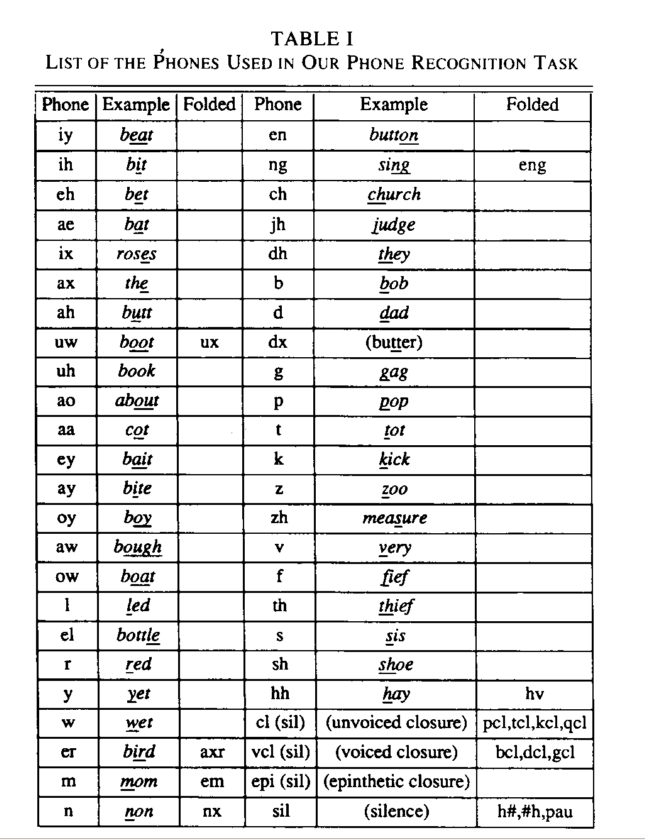
\includegraphics[width=0.7\linewidth]{../png/phoneTable}
\caption{48 to 39 phoneme folding as shown in \cite{Lee1989}.}
\label{fig:phoneTable}
\end{figure}

For all experiments the timit data set is split into a training, validation and test set. Containing 3696, 400 and 192 sentences \cite[page  80]{Graves2012}.  


\section{BLSTM-CTC}
This section explores bidirectional long short term memory layers with CTC output on the timit corpus \cite{Graves2012, Graves2006}. Training began after transforming of the speech data into Mel frequency cepstral coefficients (\textit{MFCCC}s) and phoneme folding as described above. Two \textit{bLSTM} layers where stacked on top of each other. The logits computed by the two layers where then fed into a CTC  output layer, finally beam search decoding with a beam width of 100 was used for find the phoneme predictions. The whole network was optimized using momentum gradient descent with a momentum term of 0.9 \cite[page 78]{Graves2012} and a learning rate of $10^(-3)$ . To ensure generalization normal input noise $\mathcal{N}(\mu = 0,\sigma = 0.65)$ was added to the inputs. All weights where initialized using another Gaussian $\mathcal{N}(0,0.1)$. Gradients where clipped such that all gradient elements are within $(-1,1)$.
\begin{figure}
\centering
\includestandalone[width=0.7\linewidth]{../tikz/ctc2LayerBLSTMclippedGrad}
\caption{Validation and Test set error while training a two layer BLSTM network with CTC output layer on the TIMIT speech corpus with 39 folded phonemes.}
\label{fig:ctc2BLSTM41}
\end{figure}
Results of the training process are shown in figure~\ref*{fig:ctc2BLSTM41}. 

\section{PBLSTM-CTC}

